\section{分布插值}
\label{sec:ot-interpolation}

给定两个分布$\mu_0,\mu_1$，怎样在它们之间连一条路径$\mu_t$，$0\leq t\leq1$？最直接的是混合$(1-t)\mu_0+t\mu_1$：质量不动，只是把权重从一个分布渐渐挪到另一个。取$\mu_0=\delta_0$，$\mu_1=\delta_1$，混合路径在中途是$\tfrac12\delta_0+\tfrac12\delta_1$，一半质量在$0$、一半在$1$，中间位置$\tfrac12$上什么也没有。若把分布想成一堆土，更自然的中途状态是“土堆搬到了一半的路上”，即$\delta_{1/2}$。最优运输给出这种路径：沿最优耦合把每份质量匀速推向它的目的地。

\begin{definition}[位移插值]
\label{def:ot-displacement}
设$\mu_0,\mu_1$是$\mathbb{R}^{d}$上具有有限二阶矩的分布，$\pi$是它们在平方欧氏成本下的一个最优耦合。对$0\leq t\leq1$，令$e_t(x,y)=(1-t)x+ty$，称
\begin{equation}
 \mu_t=(e_t)_\#\pi
 \label{eq:ot-displacement}
\end{equation}
为沿$\pi$的\term{位移插值}（displacement interpolation）。
\end{definition}

用随机向量说，取$(X,Y)\sim\pi$，$\mu_t$就是$(1-t)X+tY$的分布：每份质量从$X$出发，沿直线匀速走到$Y$，$t$时刻走完全程的$t$。$e_0,e_1$是两个坐标投影，所以端点正是$\mu_0,\mu_1$。$(1-t)x+ty$的平方范数不超过$2\lVert x\rVert_2^{2}+2\lVert y\rVert_2^{2}$，所以$\mu_t$也有有限二阶矩。

\begin{theorem}[位移插值是常速测地线]
\label{thm:ot-geodesic}
在定义~\ref{def:ot-displacement}的条件下，对一切$0\leq s\leq t\leq1$，
\begin{equation}
 W_2(\mu_s,\mu_t)=(t-s)\,W_2(\mu_0,\mu_1).
 \label{eq:ot-geodesic}
\end{equation}
\end{theorem}

\begin{proof}
记$W=W_2(\mu_0,\mu_1)$，$(X,Y)\sim\pi$。$\bigl((1-s)X+sY,\ (1-t)X+tY\bigr)$是$\mu_s$与$\mu_t$的一个耦合，两分量之差为$(t-s)(Y-X)$，所以
\[
 W_2^{2}(\mu_s,\mu_t)\leq(t-s)^{2}\,\mathbb{E}\lVert X-Y\rVert_2^{2}=(t-s)^{2}W^{2} .
\]
同样得到$W_2(\mu_0,\mu_s)\leq sW$，$W_2(\mu_t,\mu_1)\leq(1-t)W$。由$W_2$的三角不等式（第~\ref{chap:distribution-comparison}章），
\[
 \begin{aligned}
 W&\leq W_2(\mu_0,\mu_s)+W_2(\mu_s,\mu_t)+W_2(\mu_t,\mu_1)\\
 &\leq sW+(t-s)W+(1-t)W=W .
 \end{aligned}
\]
两端相等，中间每个不等号都必须取等，于是式~\eqref{eq:ot-geodesic}成立。
\end{proof}

式~\eqref{eq:ot-geodesic}说的是：$t\mapsto\mu_t$在度量$W_2$下走的是一条最短路，并且匀速，称为常速\term{测地线}（geodesic）。沿路径任意两点之间的距离恰好等于参数之差乘以全长，路径上不存在任何绕路。

\paragraph{两个点质量}
$\delta_0$与$\delta_1$之间只有一个耦合，位移插值是$\mu_t=\delta_t$，$W_2(\mu_s,\mu_t)=t-s$。混合路径$\nu_t=(1-t)\delta_0+t\delta_1$完全不同。$\nu_s$与$\nu_t$都在$\{0,1\}$上，它们在点$1$处的质量相差$t-s$，任何耦合至少要让这么多质量在$0$与$1$之间移动距离$1$；把恰好$t-s$的质量从$0$搬到$1$就做到了，所以
\[
 W_2(\nu_s,\nu_t)=\sqrt{t-s} .
\]
它不与$t-s$成正比。把$[0,1]$等分成$n$段，混合路径各段的$W_2$长度之和是$n\cdot\sqrt{1/n}=\sqrt{n}\to\infty$：按位置度量，混合路径根本不是一条有限长的路。图~\ref{fig:ot-point-interp}(a)对比了两种中途状态。

\begin{BookInlineFigure}
 \centering
 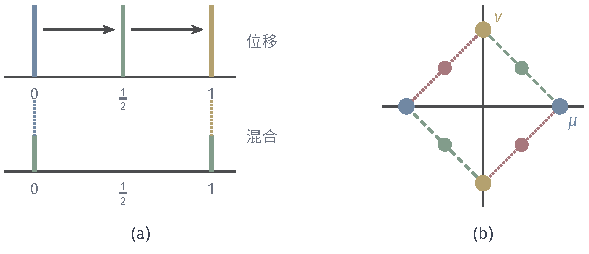
\includegraphics[width=108mm]{figures/07-probability/07-distribution-optimization/tikz/ot-point-interp/figure.pdf}
 \caption{位移插值与混合。(a)$\delta_0$（蓝）与$\delta_1$（黄）在$t=\tfrac12$的中途状态：上行是位移插值$\delta_{1/2}$，下行是混合$\tfrac12\delta_0+\tfrac12\delta_1$，竖线高度表示质量。(b)$\mu=\tfrac12(\delta_{(1,0)}+\delta_{(-1,0)})$（蓝）与$\nu=\tfrac12(\delta_{(0,1)}+\delta_{(0,-1)})$（黄），任何耦合都最优；绿色与红色分别是两个不同最优耦合的中点。}
 \label{fig:ot-point-interp}
\end{BookInlineFigure}

\paragraph{全章例子}
逐格搬运是平方成本下唯一的最优方案。$t=\tfrac12$时，留在$0$与$2$的质量不动，从$0$搬往$1$的$0.3$走到$0.5$，从$1$搬往$2$的$0.3$走到$1.5$：
\[
 \mu_{1/2}=0.2\,\delta_0+0.3\,\delta_{0.5}+0.3\,\delta_{1.5}+0.2\,\delta_2 .
\]
它与两端的距离都是$\tfrac12W_2=\tfrac12\sqrt{0.6}\approx0.387$。同一时刻的混合是$0.35\,\delta_0+0.3\,\delta_1+0.35\,\delta_2$，仍只放在原来的三个位置上。

\paragraph{一维高斯分布}
$\mu_0=\mathcal{N}(m_0,\sigma_0^{2})$与$\mu_1=\mathcal{N}(m_1,\sigma_1^{2})$之间的最优映射是$T(x)=m_1+(\sigma_1/\sigma_0)(x-m_0)$。取$X\sim\mu_0$，
\[
 (1-t)X+tT(X)=(1-t)m_0+tm_1+\Bigl((1-t)+t\frac{\sigma_1}{\sigma_0}\Bigr)(X-m_0),
\]
所以
\begin{equation}
 \mu_t=\mathcal{N}\Bigl((1-t)m_0+tm_1,\ \bigl((1-t)\sigma_0+t\sigma_1\bigr)^{2}\Bigr).
 \label{eq:ot-gaussian-geodesic}
\end{equation}
均值与标准差都线性变化，路径上始终是单峰的高斯分布。混合路径在中途是双峰的。图~\ref{fig:ot-displacement}取$m_0=-2$，$\sigma_0=0.5$，$m_1=2$，$\sigma_1=1$，画出两条路径。

\begin{BookInlineFigure}
 \centering
 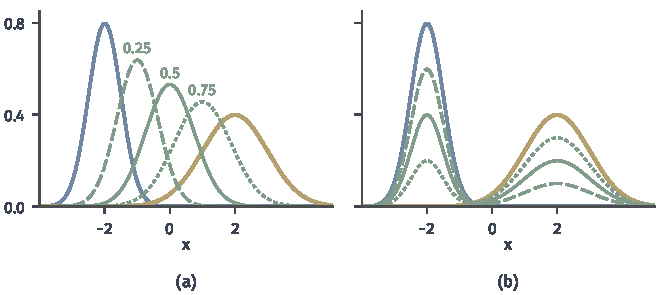
\includegraphics[width=112mm]{figures/07-probability/07-distribution-optimization/matplotlib/ot-displacement/figure.pdf}
 \caption{$\mathcal{N}(-2,0.5^{2})$（蓝）与$\mathcal{N}(2,1)$（黄）之间的两条路径，绿线是$t=0.25$（虚线）、$0.5$（实线）、$0.75$（点线）时的密度。(a)位移插值，密度整体平移并逐渐变宽。(b)混合，两个峰原地不动，只是高度此消彼长。}
 \label{fig:ot-displacement}
\end{BookInlineFigure}

\paragraph{插值不唯一}
定义~\ref{def:ot-displacement}依赖所选的最优耦合。最优耦合不唯一时，插值也不唯一。在$\mathbb{R}^{2}$中取
\[
 \mu=\tfrac12\bigl(\delta_{(1,0)}+\delta_{(-1,0)}\bigr),\qquad \nu=\tfrac12\bigl(\delta_{(0,1)}+\delta_{(0,-1)}\bigr).
\]
四个源—目标点对的平方距离都是$2$，所以每个耦合的成本都是$2$，全部最优。把$(1,0)$送到$(0,1)$、$(-1,0)$送到$(0,-1)$，中点落在$(\tfrac12,\tfrac12)$与$(-\tfrac12,-\tfrac12)$；交换目的地，中点落在另一条对角线上；独立耦合则在四个中点上各放$\tfrac14$。三者都是$\mu$与$\nu$之间的常速测地线在$t=\tfrac12$处的状态，见图~\ref{fig:ot-point-interp}(b)。

若$\mu_0$关于Lebesgue测度绝对连续，平方成本下的最优耦合唯一，并且由某个凸函数$\phi$的梯度给出：$\pi=(\mathrm{id},\nabla\phi)_\#\mu_0$。这时插值也唯一：
\[
 \mu_t=\bigl((1-t)\mathrm{id}+t\nabla\phi\bigr)_\#\mu_0 .
\]第~\ref{sec:ot-gaussian}节的对称正定线性映射就是$\phi$为二次函数的情形。一般情形的证明要用凸函数的几乎处处可微性，可查阅~\scite{math-villani2009transport}。
